\chapter{Experiment and Result}
brief of experiment and result.
\section{Experiment}
Please tell how the experiment conducted from method.

\extrafloats{100}
\maxdeadcycles=200


\section{Result}
Please provide the result of experiment

\section{Imron Sumadireja/1164076}
\subsection{Teori}
\begin{enumerate}
\item Klasifikasi Teks dan Gambar Ilustrasi \par
Klasifikasi teks merupakan sebuah model yang digunakan untuk mengkategorikan teks ke dalam kelompok-kelompok yang lebih terorganisir. Jadi untuk setiap kalimat yang di masukan ke dalam mesin, mesin tersebut akan menjadikan setiap kata dari kalimat tersebut menjadi sebuah kolom. Untuk ilustrasinya bisa dilihat pada gambar berikut \ref{Teks1}
		\begin{figure}[ht]
		\centerline{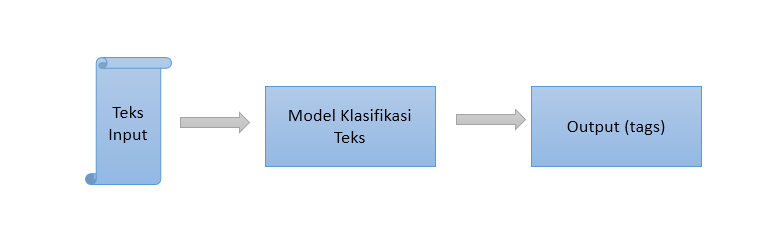
\includegraphics[width=0.5\textwidth]{figures/im/teks1.png}}
		\caption{Klasifikasi teks.}
		\label{Teks1}
		\end{figure}

\item Mengapa klasifikasi bunga tidak bisa menggunakan machine learning \par
Karena machine learning tidak dapat menampilkan inputan sesuai dengan apa yang kita inputkan. Karena inputan tersebut serupa namun mesin memberikan output yang berbeda, biasanya output atau error ini disebut dengan istilah noise. Untuk contoh sederhananya misalkan kita inputkan salah satu label yang terdapat pada bunga, output yang dihasilkan oleh mesin tersebut ialah label yang lain. Itu dikarenakan bunga banyak jenis yang serupa namun tidak sama. Untuk ilustrasinya bisa dilihat pada gambar berikut \ref{Teks2}
		\begin{figure}[ht]
		\centerline{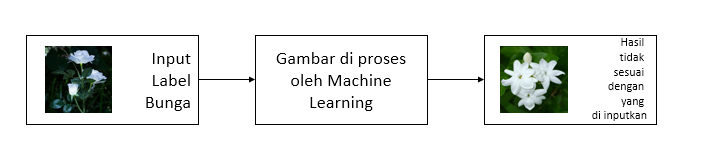
\includegraphics[width=0.5\textwidth]{figures/im/teks2.png}}
		\caption{Klasifikasi Bunga.}
		\label{Teks2}
		\end{figure}

\item Teknik pembelajaran mesin pada untuk kata-kata yang digunakan pada Youtube \par
Teknik yang digunakan pada youtube salah satunya ialah keywords. Dengan keywords tersebut mesin dapat memberikan video sesuai dengan keyword yang kita inputkan pada kolom pencarian. Teknik pembelajarannya tergantung user memberikan input teks seperti apa, karena pada youtube itu sendiri akan menyesuaikan dengan apa yang biasa kita inputkan dan akan memfilter video secara otomatis seuai dengan keyword yang biasa kita inputkan. Contoh ilustrasi sederhananya seperti berikut \ref{Teks3}
		\begin{figure}[ht]
		\centerline{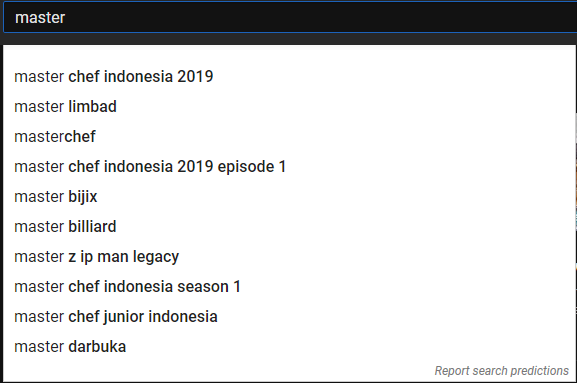
\includegraphics[width=0.5\textwidth]{figures/im/teks3.png}}
		\caption{Klasifikasi teks Youtube.}
		\label{Teks3}
		\end{figure}

\item Vektorisasi data \par
Vektorisasi data merupakan pemecahan atau pembagian data berupa teks, sebagai contoh terdapat 5 paragraf, data teks tersebut di pecah menjadi kalimat-kalimat yang lebih sederhana, lalu di pecah lagi menjadi kata untuk setiap kalimatnya. 

\item Bag of Words \par
Representasi penyederhanaan sebuah kalimat atau perhitungan setiap kata pada suatu kalimat dengan presentase berapa kali muncul kata tersebut untuk setiap kalimatnya. Contoh ilustrasi sederhananya seperti berikut \ref{Teks5}
		\begin{figure}[ht]
		\centerline{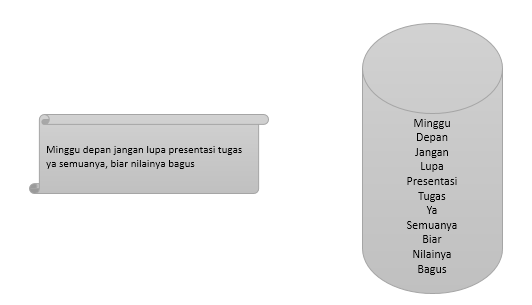
\includegraphics[width=0.5\textwidth]{figures/im/teks5.png}}
		\caption{Bag of Words.}
		\label{Teks5}
		\end{figure}

\item Apa itu TF-IDF \par
TF-IDF merupakan metode untuk menghitung bobot setiap kata pada suatu kalimat yang paling sering digunakan. TF-IDF ini akan menghitung nilai Term Frequency dan Inverse Document Frequency pada setiap kata dalam setiap kalimat yang muncul dengan diimbangi dengan jumlah dokumen dalam korpus yang mengandung kata. Contoh ilustrasi sederhananya seperti gambar berikut \ref{Teks6}
		\begin{figure}[ht]
		\centerline{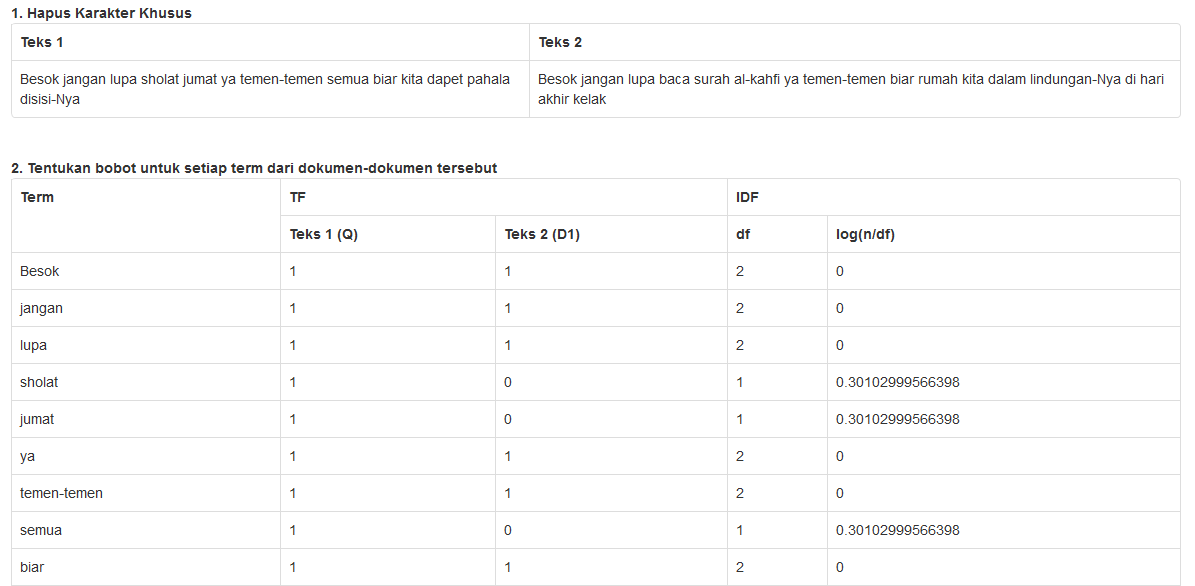
\includegraphics[width=1\textwidth]{figures/im/teks6.png}}
		\caption{TF-IDF.}
		\label{Teks6}
		\end{figure}
\end{enumerate}

\subsection{Praktikum / Imron Sumadireja / 1164076}
\begin{enumerate}
\item Buat aplikasi sederhana menggunakan pandas dengan format csv sebanyak 500 baris \par
\begin{verbatim}
import pandas as pd
d = pd.read_csv("F:/Imron/../praktikum/PraktikumChapter4/trial.csv")
\end{verbatim}
\begin{itemize}
\item Baris pertama menjelaskan import library pandas dengan inisialisasi pd untuk mengelola dataframe
\item Baris kedua untuk membaca file dengan format csv pada direktori tertentu
\item Hasilnya seperti gambar berikut \ref{df1}
\end{itemize}
		\begin{figure}[ht]
		\centerline{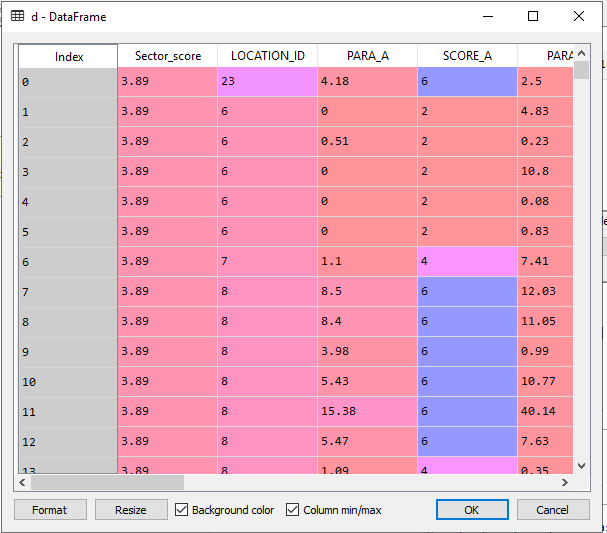
\includegraphics[width=0.5\textwidth]{figures/im/df1.png}}
		\caption{Data Frame.}
		\label{df1}
		\end{figure}

\item Memecah dataframe tersebut menjadi dua bagian yaitu 450 row pertama dan 50 row kedua \par
\begin{verbatim}
d_train=d[:450]
d_test=d[450:]
\end{verbatim}
\begin{itemize}
\item Baris pertama membagi data training menjadi 450
\item Baris kedua membagi data menjadi 50 atau sisa dari data yang tersedia
\item Hasilnya seperti gambar berikut \ref{df2}
\end{itemize}
		\begin{figure}[ht]
		\centerline{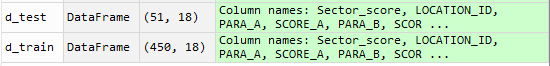
\includegraphics[width=0.5\textwidth]{figures/im/df2.png}}
		\caption{Data Frame.}
		\label{df2}
		\end{figure}

\item Praktik vektorisasi dan klasifikasi dari data katty perry dan tunjukan keluarannya
\begin{verbatim}
import pandas as pd
d = pd.read_csv("F:/Imron/../Chapter03/Youtube02-KatyPerry.csv")
\end{verbatim}
\begin{itemize}
\item Baris pertama untuk import library pandas berguna untuk mengelola dataframe
\item Baris kedua membaca file dengan format csv pada direktori tersebut
\item Untuk hasilnya seperti gambar berikut \ref{yt1}
\end{itemize}
		\begin{figure}[ht]
		\centerline{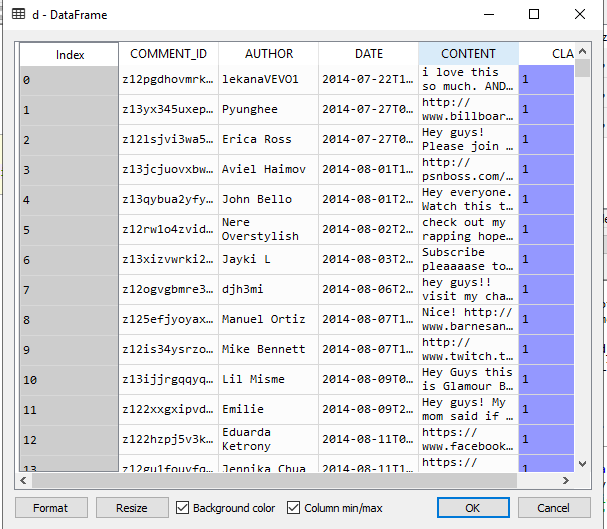
\includegraphics[width=0.5\textwidth]{figures/im/yt1.png}}
		\caption{Vektorisasi dan Klasifikasi.}
		\label{yt1}
		\end{figure}

\begin{verbatim}
spam=d.query('CLASS == 1')
nospam=d.query('CLASS == 0')
\end{verbatim}
\begin{itemize}
\item Coding tersebut untuk membagi menjadi 2 tabel spam dan nospam, untuk hasilnya seperti berikut \ref{yt2}
\end{itemize}
		\begin{figure}[ht]
		\centerline{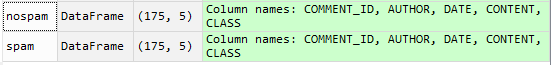
\includegraphics[width=0.5\textwidth]{figures/im/yt2.png}}
		\caption{Spam dan NoSpam.}
		\label{yt2}
		\end{figure}

\begin{verbatim}
from sklearn.feature_extraction.text import CountVectorizer
vectorizer = CountVectorizer ()
\end{verbatim}
\begin{itemize}
\item Baris pertama untuk import countvectorizer berfungsi untuk memecah data tersebut menjadi sebuah kata yang lebih sederhana
\item Baris kedua untuk menjalankan fungsi tersebut, pada code ini tidak ada hasilnya dikarenakan spyder tidak mendukung hasil dari instasiasi.
\end{itemize}

\begin{verbatim}
dvec = vectorizer.fit_transform(d['CONTENT'])
dvec
\end{verbatim}
\begin{itemize}
\item Baris pertama untuk melakukan pemecahan data pada dataframe yang terdapat pada kolom konten
\item Untuk menampilkan hasil dari code sebelumnya, hasilnya seperti gambar berikut \ref{yt3}
\end{itemize}
		\begin{figure}[ht]
		\centerline{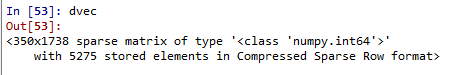
\includegraphics[width=0.5\textwidth]{figures/im/yt3.png}}
		\caption{Vektorisasi.}
		\label{yt3}
		\end{figure}

\begin{verbatim}
Daptarkata= vectorizer.get_feature_names()
\end{verbatim}
\begin{itemize}
\item Code tersebut untuk menampilkan setiap kata pada dataframe yang sudah di vektorisasi, untuk hasilnya seperti gambar berikut \ref{yt4}
\end{itemize}
		\begin{figure}[ht]
		\centerline{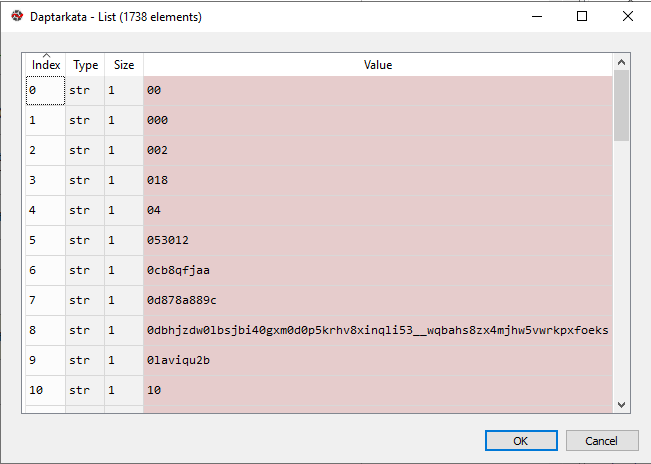
\includegraphics[width=0.5\textwidth]{figures/im/yt4.png}}
		\caption{Daftar Kata.}
		\label{yt4}
		\end{figure}

\begin{verbatim}
dshuf = d.sample(frac=1)
\end{verbatim}
\begin{itemize}
\item Code tersebut untuk mengacak dataframe tersebut agar tidak berurutan lagi sesuai dengan waktu, untuk hasilnya seperti gambar berikut \ref{yt5}
\end{itemize}
		\begin{figure}[ht]
		\centerline{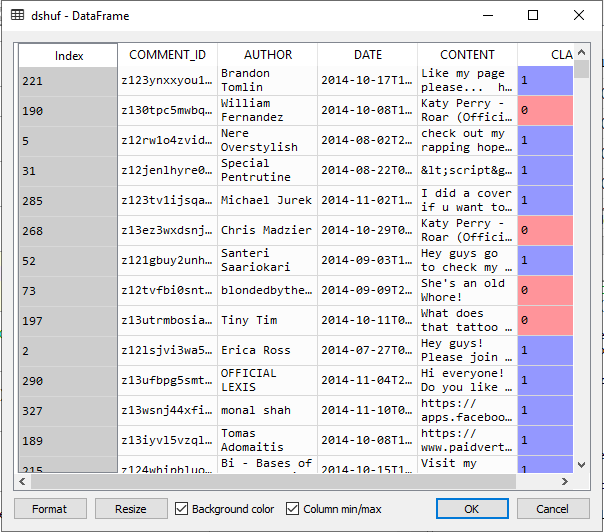
\includegraphics[width=0.5\textwidth]{figures/im/yt5.png}}
		\caption{Vektorisasi.}
		\label{yt5}
		\end{figure}

\begin{verbatim}
d_train=dshuf[:300]
d_test=dshuf[300:]
\end{verbatim}
\begin{itemize}
\item Code tersebut untuk membagi data menjadi data training dan data testing, hasilnya seperti gambar berikut \ref{yt6}
\end{itemize}
		\begin{figure}[ht]
		\centerline{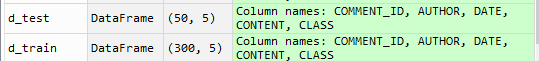
\includegraphics[width=0.5\textwidth]{figures/im/yt6.png}}
		\caption{Pembagian data training dan testing.}
		\label{yt6}
		\end{figure}

\begin{verbatim}
d_train_att = vectorizer.fit_transform(d_train['CONTENT'])
d_train_att
\end{verbatim}
\begin{itemize}
\item Baris pertama untuk memecah data pada tabel training di kolom content dari setiap kalimat menjadi kata
\item Untuk menampilkan hasil dari code tersebut
\item Hasilnya seperti gambar berikut \ref{yt7}
\end{itemize}
		\begin{figure}[ht]
		\centerline{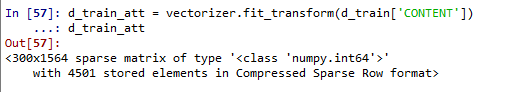
\includegraphics[width=0.5\textwidth]{figures/im/yt7.png}}
		\caption{Pemecahan data pada table training.}
		\label{yt7}
		\end{figure}

\begin{verbatim}
d_test_att=vectorizer.transform(d_test['CONTENT'])
d_test_att
\end{verbatim}
\begin{itemize}
\item Baris pertama untuk memecah data pada table testing di kolom content dari setiap kalimatnya menjadi kata
\item Untuk menampilkan hasil dari code tersebut
\item Hasilnya seperti gambar berikut \ref{yt8}
\end{itemize}
		\begin{figure}[ht]
		\centerline{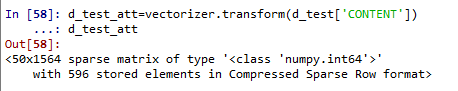
\includegraphics[width=0.5\textwidth]{figures/im/yt8.png}}
		\caption{Pemecahan data pada table testing.}
		\label{yt8}
		\end{figure}

\begin{verbatim}
d_train_label=d_train['CLASS']
d_test_label=d_test['CLASS']
\end{verbatim}
\begin{itemize}
\item Baris pertam untuk menampilkan kolom class dari data training
\item Baris kedua untuk menampilkan kolom class dari data testing
\item Hasilnya seperti gambar berikut \ref{yt9} dan \ref{yt10}
\end{itemize}
		\begin{figure}[ht]
		\centerline{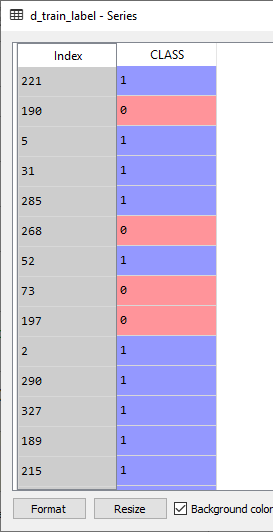
\includegraphics[width=0.5\textwidth]{figures/im/yt9.png}}
		\caption{Menampilkan kolom class.}
		\label{yt9}
		\end{figure}

		\begin{figure}[ht]
		\centerline{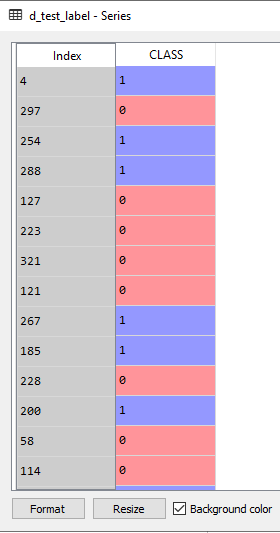
\includegraphics[width=0.5\textwidth]{figures/im/yt10.png}}
		\caption{Menampilkan kolom class.}
		\label{yt10}
		\end{figure}

\item Klasifikasi dari data vektorisasi menggunakan klasifikasi SVM \par
\begin{verbatim}
from sklearn import svm
clfsvm = svm.SVR(gamma = 'auto')
clfsvm.fit(d_train_att, d_train_label)
clfsvm.score(d_test_att, d_test_label)
\end{verbatim}
\begin{itemize}
\item Baris pertama untuk import method svm dari library sklearn
\item Nilai gamma ini berfungsi untuk memperhitungkan perolehan presentase akhir agar lebih baik
\item Untuk menyatukan data training atribut dengan label untuk di latih menggunakan metode svm
\item Untuk memunculkan score dari hasil latihan tersebut, latihan ini sama seperti k-fold dengan menggunakan 2 data
\item Hasilnya seperti gambar berikut \ref{yt11}
\end{itemize}
		\begin{figure}[ht]
		\centerline{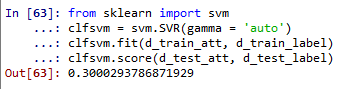
\includegraphics[width=0.5\textwidth]{figures/im/yt11.png}}
		\caption{SVM.}
		\label{yt11}
		\end{figure}

\item Klasifikasi dari data vektorisasi menggunakan klasifikasi Decision Tree \par
\begin{verbatim}
from sklearn import tree
clftree = tree.DecisionTreeClassifier()
clftree.fit(d_train_att, d_train_label)
clftree.score(d_test_att, d_test_label)
\end{verbatim}
\begin{itemize}
\item Baris pertama untuk import metode tree pada library sklearn
\item Baris kedua menjalankan decision tree classifier pada metode tree
\item Untuk menyatukan data training label dan atribut untuk dilatih menggunakan metode decision tree
\item Untuk memunculkan score dari hasil latihan dengan menggunakan metode decision tree
\item Hasilnya seperti berikut \ref{yt12}
\end{itemize}
		\begin{figure}[ht]
		\centerline{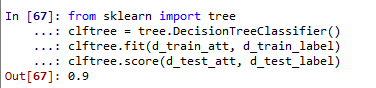
\includegraphics[width=0.5\textwidth]{figures/im/yt12.png}}
		\caption{Decision Tree.}
		\label{yt12}
		\end{figure}

\item Plotlah confusion matrix dari praktik modul ini menggunakan matplotlib \par
\begin{verbatim}
from sklearn.metrics import confusion_matrix
pred_labels=clf.predict(d_test_att)
cm=confusion_matrix(d_test_label,pred_labels)
\end{verbatim}
\begin{itemize}
\item Baris pertama untuk import metode confusion matrix pada library sklearn.metrics
\item Baris kedua menjelaskan bahwa data testing atribut akan di jalankan untuk di normalisasikan
\item Baris ketiga akan menjalankan data testing label dan data testing atribut untuk di normalisasikan pada step selanjutnya, dan code tersebut tidak mengeluarkan hasil apa-apa dikarenakan code tersebut hanya mempersiapkan data
\end{itemize}

\begin{verbatim}
import matplotlib.pyplot as plt

def plot_confusion_matrix(cm, classes,
                          normalize=False,
                          title='Confusion matrix',
                          cmap=plt.cm.Blues):
 
    if normalize:
        cm = cm.astype('float') / cm.sum(axis=1)[:, np.newaxis]
        print("Normalized confusion matrix")
    else:
        print('Confusion matrix, without normalization')

    print(cm)
\end{verbatim}
\begin{itemize}
\item Baris pertama untuk import library matplotlib dengan inisalisasi plt
\item Fungsi dari plot confusion matrix ini menormalisasikan atau menyiapkan data untuk ditampilkan berupa grafik, untuk hasilnya seperti berikut \ref{yt13} maksudnya data tersebut di prediksi ada 26 data yang termasuk bukan spam dan memang bukan spam namun ada 1 data yang di prediksi bukan spam tetapi hasilnya spam, begitupun sebaliknya terdapat 22 prediksi data spam dan itu memang termasuk dalam kategori spam tetapi ada 1 data yang di prediksi merupakan spam namun hasilnya bukan spam.
\end{itemize}
		\begin{figure}[ht]
		\centerline{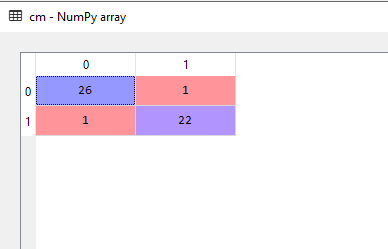
\includegraphics[width=0.5\textwidth]{figures/im/yt13.png}}
		\caption{Confusion Matrix.}
		\label{yt13}
		\end{figure}

\item Menjalankan program cross validation
\begin{verbatim}
from sklearn.model_selection import cross_val_score
scores=cross_val_score(clf,d_train_att,d_train_label,cv=5)

skor_rata2=scores.mean()
skoresd=scores.std()
\end{verbatim}
\begin{itemize}
\item Baris pertama untuk import metode cross validation
\item Melatih data training atribut dan label dengan menggunakan cross validation atau hampir sama dengan k-vold
\item Untuk menampilkan hasil dari cross validation tersebur, seperti gambar berikut \ref{yt14}
\end{itemize}
		\begin{figure}[ht]
		\centerline{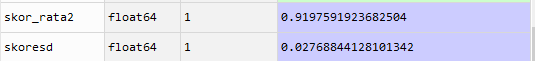
\includegraphics[width=0.5\textwidth]{figures/im/yt14.png}}
		\caption{Cross Validation.}
		\label{yt14}
		\end{figure}

\begin{verbatim}
from sklearn.model_selection import cross_val_score
scores = cross_val_score(clf, d_train_att, d_train_label, cv=5)
# show average score and +/- two standard deviations away (covering 95 \% of scores)
print("Accuracy: \%0.2f (+/-\%0.2f)" \% (scores.mean(), scores.std() * 2))
\end{verbatim}
\begin{itemize}
\item Code tersebut akan menentukan akurasi menggunakan cross validation dari hasil akurasi yang model decision tree, hasilnya seperti gambar berikut \ref{yt15}
\end{itemize}
		\begin{figure}[ht]
		\centerline{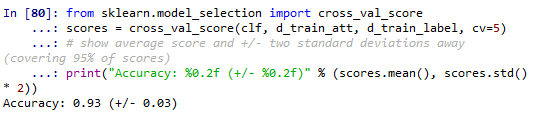
\includegraphics[width=0.5\textwidth]{figures/im/yt15.png}}
		\caption{Cross Validation.}
		\label{yt15}
		\end{figure}

\item Buatlah program pengamatan komponen informasi\par
\begin{verbatim}
max_features_opts = range(1, 10, 1)
n_estimators_opts = range(2, 40, 4)
rf_params = np.empty((len(max_features_opts)*len(n_estimators_opts),4), float)
i = 0
for max_features in max_features_opts:
    for n_estimators in n_estimators_opts:
        clf = RandomForestClassifier(max_features=max_features, n_estimators=n_estimators)
        scores = cross_val_score(clf, d_train_att, d_train_label, cv=5)
        rf_params[i,0] = max_features
        rf_params[i,1] = n_estimators
        rf_params[i,2] = scores.mean()
        rf_params[i,3] = scores.std() * 2
        i += 1
        print("Max features: \%d, num estimators: \%d, accuracy: \%0.2f (+/- \%0.2f)" \%               
              (max_features, n_estimators, scores.mean(), scores.std() * 2))
\end{verbatim}
\begin{itemize}
\item Code tersebut menjelaskan bahwa hasil dari data cross validation sebelumnya yang telah dilakukan pelatihan. Untuk range pada max features ini berfungsi untuk menampilkan parameter dari data sebelumnya dan untuk yang estimator berfungsi untuk mengatur akurasi pada gambar yang akan ditampilkan. Code tersebut tidak menampilkan keluaran
\end{itemize}

\begin{verbatim}
import matplotlib.pyplot as plt
from mpl_toolkits.mplot3d import Axes3D
from matplotlib import cm
fig = plt.figure()
fig.clf()
ax = fig.gca(projection='3d')
x = rf_params[:,0]
y = rf_params[:,1]
z = rf_params[:,2]
ax.scatter(x, y, z)
ax.set_zlim(0.9, 1)
ax.set_xlabel('Max features')
ax.set_ylabel('Num estimators')
ax.set_zlabel('Avg accuracy')
plt.show()
\end{verbatim}
\begin{itemize}
\item Code tersebut akan menampilkan grafik seperti berikut \ref{yt16} grafik tersebut dihasilkan dari data-data yang telah dilatih sebelumnya dengan menggunakan algoritma decision tree, cross validation, svm. Untuk codingan diatas pada baris kedua itu untuk import axes 3D yang berfungsi untuk menampilkan grafik 3D lalu untuk baris ke 11 itu diartikan rata-rata akurasi yang didapatkan pada pelatihan sebelumnya yang sudah dilakukan.
\end{itemize}
		\begin{figure}[ht]
		\centerline{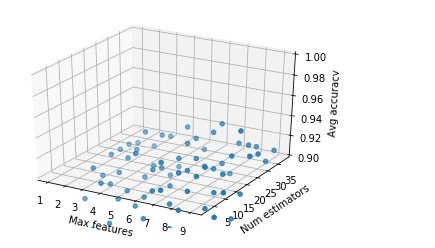
\includegraphics[width=0.5\textwidth]{figures/im/yt16.png}}
		\caption{Komponen Informasi.}
		\label{yt16}
		\end{figure}
\end{enumerate}

\section{Penanganan Error}
\subsection{Imron Sumadireja /1164076}
Hasil praktikum yang telah saya lakukan terdapat beberapa kendala error diantaranya sebagai berikut: \par
\begin{enumerate}
\item Screenshot error \ref{ytError1}
		\begin{figure}[ht]
		\centerline{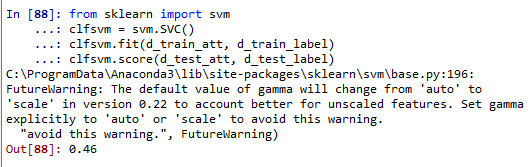
\includegraphics[width=0.5\textwidth]{figures/im/yterror1.png}}
		\caption{Screenshot error.}
		\label{ytError1}
		\end{figure}

\item Error tersebut bermasalah dengan codingan yang seharusnya SVR, itu dikarenakan pada versi spyder yang saya gunakan SVC ini tidak dapat dirunning, walaupun di running itu akan menampilkan warning. Untuk menghilangkan warning maka solusi yang saya dapatkan seperti berikut \ref{ytSolusi1}
		\begin{figure}[ht]
		\centerline{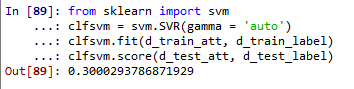
\includegraphics[width=0.5\textwidth]{figures/im/ytsolusi.png}}
		\caption{Solusi error.}
		\label{ytSolusi1}
		\end{figure}
\end{enumerate}

\section{Yusniar Nur Syarif Sidiq/1164089}
\subsection{Teori / Yusniar Nur Syarif Sidiq / 1164089}

\begin{enumerate}
\item Jelaskan apa itu klasifikasi teks, sertakan gambar ilustrasi buatan sendiri.
Klasifikasi teks merupakan sebuah proses pemberian tag atau kategori kedalam teks sesuai dengan isinya. Fungsi dari klasifikasi teks yaitu untuk melakukan klasifikasi atau pengelompokkan teks ke dalam sebuah label tertentu. Untuk contoh klasifikasi teks dapat dilihat pada figure \ref{YNC4-1}

	\begin{figure}[ht]
		\centering{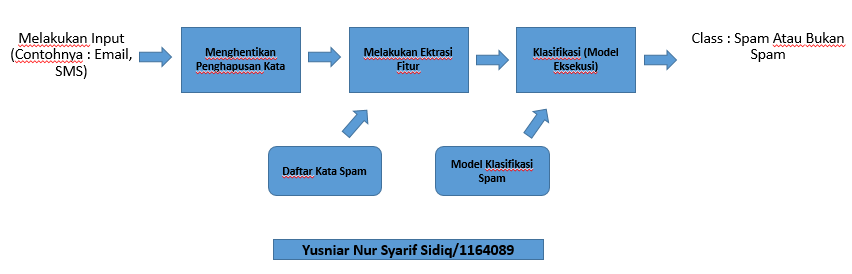
\includegraphics[scale=0.5]{figures/YN/Chapter4/YNC4-1.png}}
		\caption{Contoh Klasifikasi Teks YN}
		\label{YNC4-1}
	\end{figure}

Dimana dalam figure \ref{YNC4-1} menjelaskan terdapat daftar kata berupa kata-kata yang cukup banyak muncul pada email anda dengan tujuan menawarkan sesuatu barang atau hal lainnya, maka dapat dikategorikan bahwa kata tersebut merupakan spam.

\item Jelaskan mengapa klarifikasi bunga tidak bisa menggunakan machine learning, sertakan ilustrasi sendiri.
Karena semua bunga belum tentu memiliki ciri-ciri yang sama, atau bisa dibilang adanya data noise dalam klasifikasi bunga yang dapat menyebabkan tidak bisa menggunakan Machine Learning. Akan saya beri contoh berdasarkan ilustrasi saya sendiri, terdapat bunga mawar bewarna merah yang memiliki jumlah 5 kelopak, lalu terdapat bunga selain mawar yang  berwarna merah dan memiliki jumlah kelopak yang sama yaitu 5 serta memiliki kategori yang cukup banyak. Lalu terdapat bunga yang tidak cukup jelas datanya baik warnanya maupun jumlah kelopaknya, data tersebut akan menyababkan data noise. Untuk ilustrasi gambar akan saya berikan 2 buah gambar bunga dengan warna yang sama akan tetapi jenis yang berbeda, dapat dilihat pada figure \ref{YNC4-2}

	\begin{figure}[ht]
		\centering{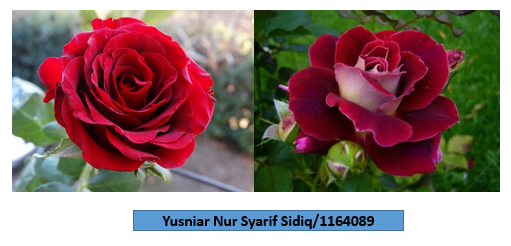
\includegraphics[scale=0.5]{figures/YN/Chapter4/YNC4-2.png}}
		\caption{Contoh Klasifikasi Bunga YN}
		\label{YNC4-2}
	\end{figure}

\item Jelaskan bagaimana teknik pembelajaran mesin pada teks pada kata-kata yang digunakan di youtube
Dapat menggunakan teknik bag-of-words pada klasifikasi berbasis text dan kata guna mengklasifikasikan sebuah komentar yang ada dalam internet sebagai kata spam atau bukan. Contohnya pada kolom komentar dapat di cek seberapa sering kata yang muncul dalam kalimat. Setiap kata bisa disebut sebagai baris dan kolomnya, hal ini merupakan dimana kategori kata spam atau tidak. Untuk ilustrasi gambarnya dapat dilihat pada figure \ref{YNC4-3}

	\begin{figure}[ht]
		\centering{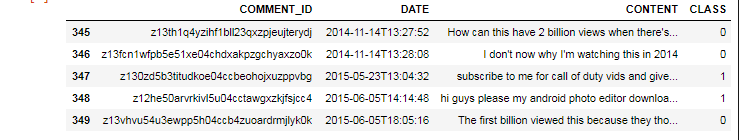
\includegraphics[scale=0.5]{figures/YN/Chapter4/YNC4-3.png}}
		\caption{Teknik Pembelajaran Mesi Pada Teks Youtube YN}
		\label{YNC4-3}
	\end{figure}


\item Jelaskan apa yang dimaksud vektorisasi data.
Vektorisasi data merupakan pembagian dan pemecahan data lalu data tersebut akan dilakukan perhitungan. Vektorisasi dapat kita maksudkan setiap data yang mungkin kita petakan ke integer tertentu. Misalnya saja kita memiliki data array yang cukup besar maka setiap kata cocok dengan slot unik dalam array. Contoh kita memiliki banyak kata yang tersesun dengan beberapa paragraf, data tersebut nantinya akan kita pecah mejadi bebera kata dalam tiap kalimatnya.

\item Jelaskan apa itu bag of words dengan kata-kata yang sederhana dan ilustrasi sendiri
bag-of-words adalah representasi penyederhanaan yang digunakan dalam pemrosesan bahasa alami dan pengambilan informasi. Model bag-of-words sederhana untuk dipahami dan diterapkan dan telah melihat kesuksesan besar dalam masalah seperti pemodelan bahasa dan klasikasi dokumen. Ilustrasinya yaitu terdapat satu kalimat dan kalimat tersebut akan dipecah menjadi kata per kata, untuk lebih jelasnya dapat dilihat pada figure \ref{YNC4-4}

	\begin{figure}[ht]
		\centering{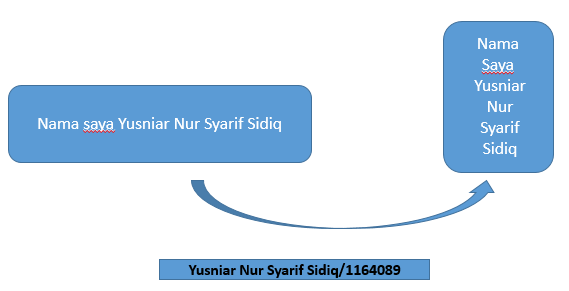
\includegraphics[scale=0.5]{figures/YN/Chapter4/YNC4-4.png}}
		\caption{Bag Of Words YN}
		\label{YNC4-4}
	\end{figure}

\item Jelaskan apa itu TF-IDF, ilustrasikan dengan gambar sendiri
TF-IDF dapat memberikan kita frekuensi kata dalam setiap dokumen sehingga dapat menggantikan data menjadi number. TD-IDF merupakan sebuah metode untuk dapat menghitung bobot setiap kata dalam kalimat yang sering digunakan. Untuk lebih jelasnya dapat dilihat dari figure \ref{TNC4-5}

	\begin{figure}[ht]
		\centering{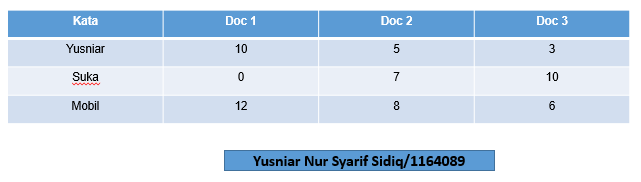
\includegraphics[scale=0.5]{figures/YN/Chapter4/YNC4-5.png}}
		\caption{TF-IDF YN}
		\label{YNC4-5}
	\end{figure}


\end{enumerate}

\subsection{Praktek Program / Yusniar Nur Syarif Sidiq / 1164089}
\begin{enumerate}

\item Buat data dummy dengan format csv sebanyak 500 baris dan melakukan load ke dataframe pandas. Jelaskan arti setiap baris kode yang dibuat.

	\begin{verbatim}
		import pandas as pd
		yn = pd.read_csv("AttributeDataSet.csv")
	\end{verbatim}

Dimana pada baris pertama akan melakukan import pandas yang di rename menjadi pd. Pada baris kedua kita akan membuat variabel yn lalu di isikan dengan file csv nya. Untuk hasil output dalam spyder bisa dilihat pada figure \ref{YNC4-6}

	\begin{figure}[ht]
		\centering{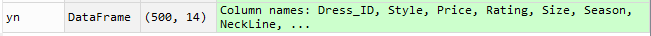
\includegraphics[scale=0.5]{figures/YN/Chapter4/No1-2/YNC4-6.png}}
		\caption{Import DataFrame 500 Baris}
		\label{YNC4-6}
	\end{figure}

\item Dari DataFrame tersebut dipecah menjadi dua DataFrame yaitu 450 row pertama dan 50 row sisanya.

	\begin{verbatim}
		d_train=yn[:450]
		d_test=yn[450:]
	\end{verbatim}

Dimana pada baris pertama menjelaskan bahwa akan membagi data traning sebanyak 450. Pada baris kedua akan membuat data testing sebanyak 50 yang merupakan sisanya. Untuk hasil output dalam spyder bisa dilihat pada figure \ref{YNC4-7}

	\begin{figure}[ht]
		\centering{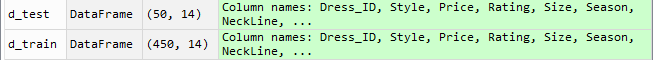
\includegraphics[scale=0.5]{figures/YN/Chapter4/No1-2/YNC4-7.png}}
		\caption{Membagi Data Menjadi 2 DataFrame}
		\label{YNC4-7}
	\end{figure}

\item Praktekan vektorisasi dan klarifikasi dari data (NPM mod 4, jika 0 maka katty perry, 1 LMFAO, 2 Eminem, 3 Shakira). Tunjukan keluarannya dari komputer sendiri dan artikan maksud setiap keluaran yang di dapatkan.

	\begin{verbatim}
		import pandas as pd
		yn=pd.read_csv("Youtube03-LMFAO.csv")
	\end{verbatim}

Dimana hasil dari output tersebut akan membaca data csv yaitu Youtube03-LMFAO. Untuk hasil output dalam spyder bisa dilihat pada figure \ref{YNC4-8}

	\begin{figure}[ht]
		\centering{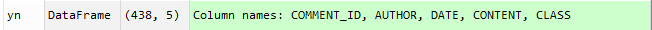
\includegraphics[scale=0.5]{figures/YN/Chapter4/C4No3/YNC4-8.png}}
		\caption{Membaca File csv}
		\label{YNC4-8}
	\end{figure}	

Selanjutnya perhatikan source code dibawah ini,

	\begin{verbatim}
		spam=yn.query('CLASS == 1')
		nospam=yn.query('CLASS == 0')
	\end{verbatim}	

Dimana pada source code tersebut akan membagi data spam dan bukan spam, yang berarti data spam akan diberi tanda 1 dan data yang bukan spam akan diberi tanda 0. Untuk hasil output dalam spyder bisa dilihat pada figure \ref{YNC4-9}

	\begin{figure}[ht]
		\centering{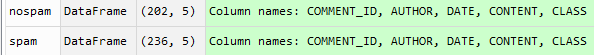
\includegraphics[scale=0.5]{figures/YN/Chapter4/C4No3/YNC4-9.png}}
		\caption{Membagi Data Spam Dan Bukan Spam}
		\label{YNC4-9}
	\end{figure}	

Lanjut ke source code berikutnya,

	\begin{verbatim}
		from sklearn.feature_extraction.text import CountVectorizer
		vectorizer = CountVectorizer()
	\end{verbatim}	

Dimana source code diatas akan memanggil lib vektorisasi dan akan melakukan fungsi bag of word yaitu menghitung kata yang muncul perkalimat. Untuk hasil output dalam spyder bisa dilihat pada figure \ref{YNC4-10}

	\begin{figure}[ht]
		\centering{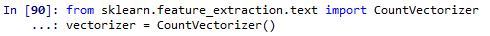
\includegraphics[scale=0.5]{figures/YN/Chapter4/C4No3/YNC4-10.png}}
		\caption{Fungsi Bag Of Word}
		\label{YNC4-10}
	\end{figure}

Selanjutnya perhatikan source code berikut,

	\begin{verbatim}
		dvec = vectorizer.fit_transform(yn['CONTENT'])
		dvec
	\end{verbatim}	

Dimana pada source code tersebut akan melakukan vektorisasi pada colom content dan akan ditampilkan hasilnya. Untuk output dalam spyder dapat dilihat pada figure \ref{YNC4-11}

	\begin{figure}[ht]
		\centering{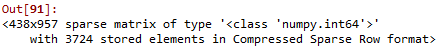
\includegraphics[scale=0.5]{figures/YN/Chapter4/C4No3/YNC4-11.png}}
		\caption{Melakukan Vektorisasi Pada Colom Content}
		\label{YNC4-11}
	\end{figure}

Lanjut ke source code berikutnya,

	\begin{verbatim}
		dk=vectorizer.get_feature_names()
	\end{verbatim}

Dimana pada source code tersebut akan menampilkan data yang sudah di vektorisasi. Untuk output dalam spyder dapat dilihat pada figure \ref{YNC4-12}

	\begin{figure}[ht]
		\centering{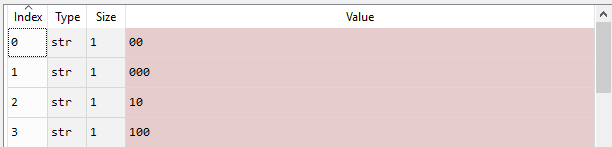
\includegraphics[scale=0.5]{figures/YN/Chapter4/C4No3/YNC4-12.png}}
		\caption{Data Yang Sudah Di Vektorisasi}
		\label{YNC4-12}
	\end{figure}

Selanjutnya perhatikan source code dibawah,

	\begin{verbatim}
		yeay = yn.sample(frac=1)
	\end{verbatim}

Dimana pada source code tersebut akan melakukan pengacakan data pada database agar sempurna saat akan melakukan klasifikasi. Untuk output dalam spyder dapat dilihat pada figure \ref{YNC4-13}

	\begin{figure}[ht]
		\centering{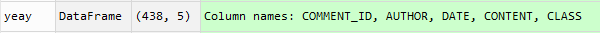
\includegraphics[scale=0.5]{figures/YN/Chapter4/C4No3/YNC4-13.png}}
		\caption{Pengacakan Data}
		\label{YNC4-13}
	\end{figure}

Lanjut ke source code berikutnya,

	\begin{verbatim}
		yn_train=yeay[:300]
		yn_test=yeay[300:]
	\end{verbatim}

Dimana pada source code tersebut akan membagi menjadi 2 DataFrame yaitu 300 pada data training dan sisanya data testing. Untuk output dalam spyder dapat dilihat pada figure \ref{YNC4-14}

	\begin{figure}[ht]
		\centering{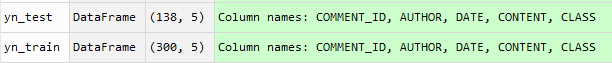
\includegraphics[scale=0.5]{figures/YN/Chapter4/C4No3/YNC4-14.png}}
		\caption{Membagi Data Yang Sudah Di Vektorisasi}
		\label{YNC4-14}
	\end{figure}

Selanjutnya perhatikan source code dibawah,

	
	\begin{verbatim}
		yn_train_att=vectorizer.fit_transform(yn_train['CONTENT'])
		yn_train_att
	\end{verbatim}

Dimana akan dilakukannya training pada data training dan akan di vektorisasi.  Untuk output dalam spyder dapat dilihat pada figure \ref{YNC4-15}

	\begin{figure}[ht]
		\centering{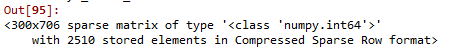
\includegraphics[scale=0.5]{figures/YN/Chapter4/C4No3/YNC4-15.png}}
		\caption{Vektorisasi Pada Data Training}
		\label{YNC4-15}
	\end{figure}

Selanjutnya perhatikan source code dibawah,

	
	\begin{verbatim}
		yn_test_att=vectorizer.transform(yn_test['CONTENT'])
		yn_test_att
	\end{verbatim}

Dimana akan dilakukannya testing pada data testing dan akan di vektorisasi.  Untuk output dalam spyder dapat dilihat pada figure \ref{YNC4-16}

	\begin{figure}[ht]
		\centering{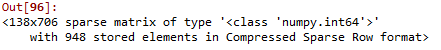
\includegraphics[scale=0.5]{figures/YN/Chapter4/C4No3/YNC4-16.png}}
		\caption{Vektorisasi Pada Data Testing}
		\label{YNC4-16}
	\end{figure}

Lanjut ke source code berikut ini,

	\begin{verbatim}
		yn_train_label=yn_train['CLASS']
		yn_test_label=yn_test['CLASS']
	\end{verbatim}

Dimana pada source code tersebut akan mengambil data spam dan bukan spam dari data training dan testing. Untuk output dalam spyder dapat dilihat pada figure \ref{YNC4-17}

	\begin{figure}[ht]
		\centering{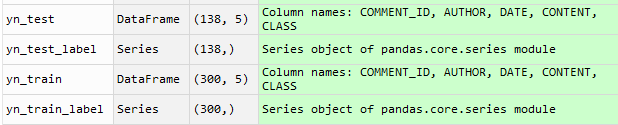
\includegraphics[scale=0.5]{figures/YN/Chapter4/C4No3/YNC4-17.png}}
		\caption{Mengambil Data Spam Dan Bukan Dari Traning Dan Testing Data}
		\label{YNC4-17}
	\end{figure}

\item Cobalah klasifikasikan dari data vektorisasi yang di tentukan di nomor sebelumnya dengan klasifikasi SVM.

	\begin{verbatim}
		from sklearn import svm
		clfsvm = svm.SVR(gamma='auto')
		clfsvm.fit(yn_train_att, yn_train_label)
		clfsvm.score(yn_test_att, yn_test_label)
	\end{verbatim}

Dimana pada source code tersebut akan melakukan import svm dari library sklearn dan akan melakukan klasifikasi dari data yang sudah di vektorisasikan. Hasil output dari source code tersebut berupa score prediksi dari svm. Untuk output dalam spyder dapat dilihat pada figure \ref{YNC4-18}

	\begin{figure}[ht]
		\centering{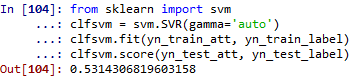
\includegraphics[scale=0.5]{figures/YN/Chapter4/C4No4/YNC4-18.png}}
		\caption{Score Prediksi Dari SVM}
		\label{YNC4-18}
	\end{figure}

\item Cobalah klasifikasikan dari data vektorisasi yang di tentukan nomor sebelumnya dengan klasifikasi Decision Tree.

	\begin{verbatim}
		from sklearn import tree
		clftree = tree.DecisionTreeClassifier()
		clftree.fit(yn_train_att, yn_train_label)
		clftree.score(yn_test_att, yn_test_label)
	\end{verbatim}

Dimana source code tersebut akan melakukan import modul tree dari library sklearn dan akan melakukan klasifikasi dari data yang sudah di vektorisasikan. Hasil dari output source code tersebut akan berupa score dari prediksi Decision Tree. Untuk output dalam spyder dapat dilihat pada figure \ref{YNC4-19}

	\begin{figure}[ht]
		\centering{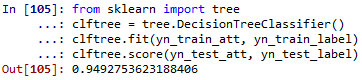
\includegraphics[scale=0.5]{figures/YN/Chapter4/C4No5/YNC4-19.png}}
		\caption{Score Prediksi Dari Decision Tree}
		\label{YNC4-19}
	\end{figure}

\item Plotlah confusion matrix dari praktek modul ini menggunakan matplotlib.

	\begin{verbatim}
		import matplotlib.pyplot as plt

		def plot_confusion_matrix(cm, classes,
                         	 normalize=False,
                         	 title='Confusion matrix',
                         	 cmap=plt.cm.Blues):
  		  """
   		 This function prints and plots the confusion matrix.
   		 Normalization can be applied by setting `normalize=True`.
 		   """
   		 if normalize:
       			 cm = cm.astype('float') / cm.sum(axis=1)[:, np.newaxis]
     	   		 print("Normalized confusion matrix")
    		else:
        			print('Confusion matrix, without normalization')

   		 print(cm)
	\end{verbatim}

Dalam source code tersebut akan melakukan import library matplotlib dan di rename menjadi plt lalu memasukkan fungsi confusion matrix. Untuk output dalam spyder dapat dilihat pada figure \ref{YNC4-20}

	\begin{figure}[ht]
		\centering{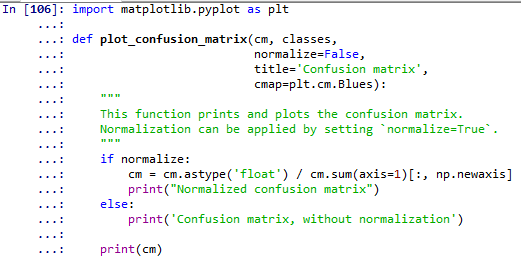
\includegraphics[scale=0.5]{figures/YN/Chapter4/C4No6/YNC4-20.png}}
		\caption{Import Matplotlib}
		\label{YNC4-20}
	\end{figure}

Selanjutnya perhatikan source code berikut ini,

	\begin{verbatim}
		import numpy as np
		np.set_printoptions(precision=2)
		plot_confusion_matrix(cm, classes=yn, normalize=True)
		plt.show()
	\end{verbatim}

Dimana pada soirce code tersebut akan melakukan import pada library numpy yang dimana akan di rename menjadi np. Numpy disini berfungsi sebagai pengolah data matix arti dari numpy sendiri yaitu numarical matrix. Hasil dari source code tersebut akan memunculkan data matrix yang sudah di normalisasi. Untuk output dalam spyder dapat dilihat pada figure \ref{YNC4-21}

	\begin{figure}[ht]
		\centering{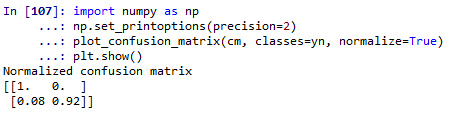
\includegraphics[scale=0.5]{figures/YN/Chapter4/C4No6/YNC4-21.png}}
		\caption{Matrix Normalisasi}
		\label{YNC4-21}
	\end{figure}

\item Jalankan program cross validation.

	\begin{verbatim}
		from sklearn.model_selection import cross_val_score
		scores = cross_val_score(clf, yn_train_att, yn_train_label, cv=5)
		print("Accurac")
	\end{verbatim}

Dimana pada source code diatas akan menampilkan score akurasi pada Random Forest. Untuk output dalam spyder dapat dilihat pada figure \ref{YNC4-22}

	\begin{figure}[ht]
		\centering{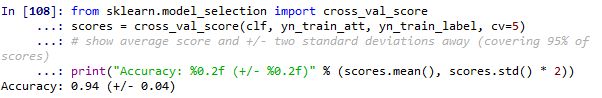
\includegraphics[scale=0.5]{figures/YN/Chapter4/C4No7/YNC4-22.png}}
		\caption{Score Prediksi Akurasi RF}
		\label{YNC4-22}
	\end{figure}

Selanjutnya perhatikan source code dibawah ini,

	\begin{verbatim}
		scorestree = cross_val_score(clftree, yn_train_att, yn_train_label, cv=5)
		print("Accuracy")
	\end{verbatim}

Dimana pada source code diatas akan menampilkan score akurasi pada Decision Tree. Untuk output dalam spyder dapat dilihat pada figure \ref{YNC4-23}

	\begin{figure}[ht]
		\centering{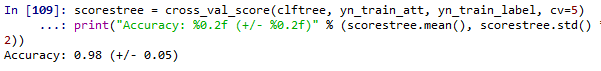
\includegraphics[scale=0.5]{figures/YN/Chapter4/C4No7/YNC4-23.png}}
		\caption{Score Prediksi Akurasi DT}
		\label{YNC4-23}
	\end{figure}

Selanjutnya perhatikan source code dibawah ini,

	\begin{verbatim}
		scoressvm = cross_val_score(clfsvm, yn_train_att, yn_train_label, cv=5)
		print("Accuracy")
	\end{verbatim}

Dimana pada source code diatas akan menampilkan score akurasi pada SVM. Untuk output dalam spyder dapat dilihat pada figure \ref{YNC4-24}

	\begin{figure}[ht]
		\centering{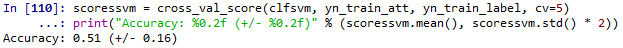
\includegraphics[scale=0.5]{figures/YN/Chapter4/C4No7/YNC4-24.png}}
		\caption{Score Prediksi Akurasi SVM}
		\label{YNC4-24}
	\end{figure}

\item Buatlah program pengamatan komponen informasi.

	\begin{verbatim}
		max_features_opts = range(1, 10, 1)
		n_estimators_opts = range(2, 40, 4)
		rf_params = np.empty((len(max_features_opts)*len(n_estimators_opts),4), float)
		i = 0
		for max_features in max_features_opts:
    		for n_estimators in n_estimators_opts:
        		clf = RandomForestClassifier(max_features=max_features, n_estimators=n_estimators)
       		 scores = cross_val_score(clf, yn_train_att, yn_train_label, cv=5)
      		 rf_params[i,0] = max_features
       		 rf_params[i,1] = n_estimators
        		rf_params[i,2] = scores.mean()
       		 rf_params[i,3] = scores.std() * 2
       		 i += 1
       		 print("Max features"
	\end{verbatim}

Output dari source code diatas akan melakukan pengulangan dari data-data sebelumnya yang sudah di vektorisasi.  Untuk output dalam spyder dapat dilihat pada figure \ref{YNC4-25}

	\begin{figure}[ht]
		\centering{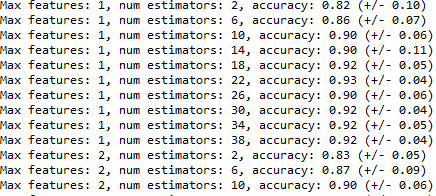
\includegraphics[scale=0.5]{figures/YN/Chapter4/C4No8/YNC4-25.png}}
		\caption{Pengulangan Data Vektorisasi}
		\label{YNC4-25}
	\end{figure}

Selanjutnya perhatikan source code berikut,

	\begin{verbatim}
		import matplotlib.pyplot as plt
		from mpl_toolkits.mplot3d import Axes3D
		from matplotlib import cm
		fig = plt.figure()
		fig.clf()
		ax = fig.gca(projection='3d')
		x = rf_params[:,0]
		y = rf_params[:,1]
		z = rf_params[:,2]
		ax.scatter(x, y, z)
		ax.set_zlim(0.8, 1)
		ax.set_xlabel('Max features')
		ax.set_ylabel('Num estimators')
		ax.set_zlabel('Avg accuracy')
		plt.show()
	\end{verbatim}

Hasil output dari source code tersebut adalh menampilkan data pengulangan yang sudah di vektorisasi dalam bentuk grafik. Untuk output dalam spyder dapat dilihat pada figure \ref{YNC4-26}

	\begin{figure}[ht]
		\centering{\includegraphics[scale=0.5]{figures/YN/Chapter4/C4No8/YNC4-26.png}}
		\caption{Grafik Data Pengulangan}
		\label{YNC4-26}
	\end{figure}

\end{enumerate}

\subsection{Penangan Error / Yusniar Nur Syarif Sidiq / 1164089}
\begin{enumerate}

\item Screenshoot Error
Dimana error yang saya dapat ditunjukan pada figure \ref{YNC4-27}

	\begin{figure}[ht]
		\centering{\includegraphics[scale=0.5]{figures/YN/Chapter4/C4PE/YNC4-27.png}}
		\caption{Syntax Error}
		\label{YNC4-27}
	\end{figure}

\item Tuliskan kode error dan jenisnya

	\begin{verbatim}
		from sklearn import svm
		clfsvm = svm.SVR()
		clfsvm.fit(yn_train_att, yn_train_label)
		clfsvm.score(yn_test_att, yn_test_label)
	\end{verbatim}

Dimana error tersebut merupakan syntax error yaitu terjadi kekurangan source code atau salah penulisannya.

\item Solusi pemecahan masalah error
Solusi dari error tersebut adalah dengan melengkapi source codenya. Untuk source code lengkapnya dapat dilihat dibawah ini

	\begin{verbatim}
		from sklearn import svm
		clfsvm = svm.SVR(gamma='auto')
		clfsvm.fit(yn_train_att, yn_train_label)
		clfsvm.score(yn_test_att, yn_test_label)
	\end{verbatim}

\end{enumerate}